\documentclass[aspectratio=169,11pt]{beamer}

\usetheme{metropolis}
\metroset{progressbar=frametitle, sectionpage=progressbar, numbering=none}

\usepackage[ngerman]{babel}
\usepackage{tikz}
\usetikzlibrary{arrows.meta,positioning,calc,decorations.pathreplacing,fit,backgrounds}
\usepackage{fontawesome5}

% BFH / Metropolis preamble for the WDDA regression walkthrough deck.
% Brand colours and logo handling adapted from the BSAN "litmus/bfh" theme.

% === BRAND COLORS ===
\usepackage{xcolor}
\definecolor{LitmusPrimary}{HTML}{697D91}
\definecolor{LitmusSecondary}{HTML}{FAC300}
\definecolor{LitmusAccent}{HTML}{699673}
\definecolor{LitmusDark}{HTML}{697D91}
\definecolor{LitmusCorrect}{HTML}{699673}
\definecolor{LitmusIncorrect}{HTML}{B41428}
\definecolor{LitmusAlert}{HTML}{F7931E}

% === GRAPHICS / LOGOS ===
\usepackage{graphicx}
\newcommand{\litmuslogo}{bfh-logo.pdf}
\newcommand{\litmoslockup}{bfh-lockup.pdf}

% === MATH ===
\usepackage{amsmath,amssymb}
\usepackage{booktabs}

% === CODE LISTINGS (R) ===
\usepackage{listings}
\lstdefinestyle{Rcode}{
  language=R,
  basicstyle=\ttfamily\footnotesize,
  keywordstyle=\color{LitmusAccent}\bfseries,
  commentstyle=\color{gray}\itshape,
  stringstyle=\color{LitmusPrimary},
  numberstyle=\tiny\color{gray},
  frame=single,
  framerule=0.5pt,
  rulecolor=\color{LitmusAccent!30},
  backgroundcolor=\color{LitmusDark!5},
  breaklines=true,
  showstringspaces=false,
  columns=fullflexible,
  keepspaces=true,
}
% Console-output style (no syntax colours)
\lstdefinestyle{Rout}{
  basicstyle=\ttfamily\footnotesize\color{black!80},
  frame=single,
  framerule=0.5pt,
  rulecolor=\color{LitmusPrimary!25},
  backgroundcolor=\color{LitmusPrimary!4},
  breaklines=true,
  showstringspaces=false,
}
\lstnewenvironment{rcode}{\lstset{style=Rcode}}{}
\lstnewenvironment{rout}{\lstset{style=Rout}}{}

% === METROPOLIS / BEAMER TWEAKS ===
\setbeamercolor{progress bar}{fg=LitmusSecondary}
\setbeamercolor{alerted text}{fg=LitmusAlert}
\setbeamercolor{example text}{fg=LitmusAccent}
\setbeamercolor{frametitle}{bg=LitmusPrimary}

% Footer logo on regular slides (skip the title page)
\setbeamertemplate{frame footer}{%
  \ifnum\value{page}>1\relax
    \IfFileExists{\litmuslogo}{\includegraphics[height=0.3cm]{\litmuslogo}}{}%
  \fi
}

% Title page with the BFH lockup logo
\makeatletter
\setbeamertemplate{title page}{
  \begin{minipage}[b][\paperheight]{\textwidth}
    \vfill
    \ifx\inserttitle\@empty\else\usebeamertemplate*{title}\fi
    \ifx\insertsubtitle\@empty\else\usebeamertemplate*{subtitle}\fi
    \usebeamertemplate*{title separator}
    \ifx\beamer@shortauthor\@empty\else\usebeamertemplate*{author}\fi
    \ifx\insertdate\@empty\else\usebeamertemplate*{date}\fi
    \ifx\insertinstitute\@empty\else\usebeamertemplate*{institute}\fi
    \vfill
    \IfFileExists{\litmoslockup}{\includegraphics[height=1cm]{\litmoslockup}}{}
    \vspace*{1em}
  \end{minipage}
}
\makeatother

% === CONTENT BOXES (concept / takeaway / warning) ===
\usepackage{tcolorbox}
\tcbuselibrary{skins}
\newtcolorbox{konzept}[1][Kernkonzept]{
  colback=LitmusAccent!6, colframe=LitmusAccent,
  fonttitle=\bfseries, title={#1}, boxrule=0.8pt, arc=2pt,
  left=4pt, right=4pt, top=3pt, bottom=3pt,
}
\newtcolorbox{merke}[1][Merke]{
  colback=LitmusSecondary!12, colframe=LitmusSecondary!85!black,
  fonttitle=\bfseries, title={#1}, boxrule=0.8pt, arc=2pt,
  left=4pt, right=4pt, top=3pt, bottom=3pt,
}
\newtcolorbox{warnung}[1][Achtung]{
  colback=LitmusIncorrect!6, colframe=LitmusIncorrect,
  fonttitle=\bfseries, title={#1}, boxrule=0.8pt, arc=2pt,
  left=4pt, right=4pt, top=3pt, bottom=3pt,
}


\title{Musterprüfung --- Aufgaben 15--20}
\subtitle{Schritt für Schritt zur Lösung --- WDDA FS 2026}
\author{Ulrich Matter}
\date{}
\institute{Berner Fachhochschule --- Datenmanagement und Datenanalyse}

\begin{document}

\frame{\titlepage}

% ============================================================
\begin{frame}{Worum geht es heute?}
Wir lösen \alert{sechs Prüfungsfragen} --- von der beschreibenden Statistik
bis zur Regression:

\vspace{0.3cm}
\begin{columns}[T]
\begin{column}{0.5\textwidth}
  \begin{konzept}[Fragen 15--17]
  \textbf{Beschreiben}\\[2pt]
  Boxplots zuordnen (15), Skalenniveau \& Lagemass (16), Streuung, Form
  \& Ausreisser (17).
  \end{konzept}
\end{column}
\begin{column}{0.5\textwidth}
  \begin{konzept}[Fragen 18--20]
  \textbf{Schliessen \& Modellieren}\\[2pt]
  Bootstrap-CI für eine Anteilsdifferenz (18), Streudiagramme lesen (19),
  einfache Regression (20).
  \end{konzept}
\end{column}
\end{columns}

\vspace{0.3cm}
Roter Faden: \textbf{Erst die Daten verstehen (Skalenniveau, Lage,
Streuung), dann Unsicherheit beziffern und Zusammenhänge modellieren.}
\end{frame}

\begin{frame}{Wichtiger Hinweis zur Musterprüfung}
\begin{warnung}[Mehrere Versionen pro Aufgabe]
Wie in der \textbf{echten Prüfung} gibt es zu jeder Aufgabe \alert{mehrere
Versionen} desselben Typs --- mit leicht \textbf{anderen Datensätzen bzw.\
Zahlen}, die beim Prüfungsantritt \textbf{zufällig} ausgewählt werden.
\end{warnung}

\vspace{0.2cm}
Sie bearbeiten dieselben Aufgaben wie hier --- aber Ihre \textbf{konkreten
Zahlen können abweichen}. \alert{Keine Sorge}, wenn Ihre Ergebnisse nicht
exakt mit den Werten auf diesen Folien übereinstimmen.
\end{frame}

\begin{frame}{Lernziele}
Nach diesen sechs Fragen können Sie:
\begin{enumerate}
  \item einen \alert{Boxplot lesen} und der passenden deskriptiven Statistik
        (Median, SD, Schiefe) zuordnen;
  \item die \alert{vier Skalenniveaus} unterscheiden und das passende
        \alert{Lagemass} (Modus, Median, Mittelwert) wählen;
  \item \alert{Streuung} (SD, IQR) und \alert{Form} (Schiefe) berechnen
        und \alert{Ausreisser} mit der Tukey-Regel finden;
  \item ein \alert{Bootstrap-Konfidenzintervall} für eine Anteilsdifferenz
        bestimmen und auf Signifikanz prüfen;
  \item ein \alert{standardisiertes Streudiagramm} lesen und Korrelation,
        Lage und Streuung abschätzen;
  \item eine \alert{einfache lineare Regression} schätzen, $R^2$ und das
        Konfidenzintervall der Steigung interpretieren.
\end{enumerate}
\end{frame}

% ============================================================
\section{Frage 15 --- Boxplots zuordnen}
% ============================================================

\begin{frame}{Die Aufgabe \& die Idee dahinter}
\textbf{Aufgabentyp \texttt{Zuordnung Boxplots}:} Ordnen Sie jedem Boxplot
die passende deskriptive Statistik (\texttt{Mean}, \texttt{SD},
\texttt{Median}) zu.

\vspace{0.3cm}
\begin{konzept}[Schlüssel]
Ein Boxplot zeigt \textbf{Median}, \textbf{Streuung} und \textbf{Form}
direkt --- daraus lassen sich die drei Kennzahlen ablesen bzw.\ abschätzen.
\end{konzept}

\vspace{0.2cm}
Drei Leseregeln:
\begin{enumerate}
  \item \alert{Median} $=$ die Linie in der Box --- \textbf{direkt ablesbar}.
  \item \alert{SD} $\leftrightarrow$ Streuung: breitere Box $+$ längere
        Whisker $\Rightarrow$ grössere Standardabweichung.
  \item \alert{Mean vs.\ Median} $\leftrightarrow$ Form (Schiefe): siehe
        nächste Folie.
\end{enumerate}
\end{frame}

\begin{frame}{Strategie: Form verrät Mean vs.\ Median}
\begin{center}
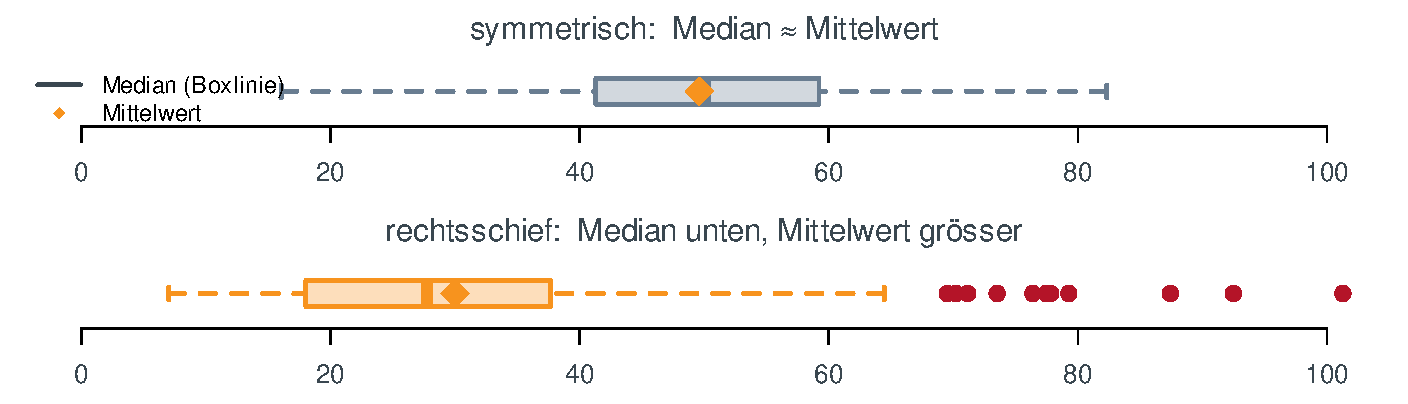
\includegraphics[width=0.76\linewidth]{figures/ex15_boxplots.pdf}
\end{center}
\vspace{0.1cm}
{\small\textbf{Vorgehen:}
\textbf{(1)}~\alert{Median} ablesen (oft schon fast eindeutig). \quad
\textbf{(2)}~\alert{Streuung} $\to$ \texttt{SD}. \quad
\textbf{(3)}~\alert{Schiefe}: Median unten $+$ Ausreisser rechts $\Rightarrow$
\texttt{Mean}$>$\texttt{Median}; symmetrisch $\Rightarrow$
\texttt{Mean}$\approx$\texttt{Median}.}

\vspace{0.15cm}
\begin{merke}[Hinweis]
\textbf{Vollständige Musterlösung} zu Frage 15: siehe \textbf{Moodle-Musterprüfung}.
\end{merke}
\end{frame}

% ============================================================
\section{Frage 16 --- Skalenniveau \& Lagemass}
% ============================================================

\begin{frame}{Die Aufgabe}
\textbf{Datensatz \texttt{Umfragedaten.xlsx}} --- 100 Personen aus einer
Marktforschungsumfrage. Vier Variablen:

\vspace{0.3cm}
\begin{enumerate}
  \item Bestimme das \alert{höchste Skalenniveau} von \texttt{Geschlecht},
        \texttt{Bildung}, \texttt{Einkommen}, \texttt{Bewertung}.
  \item Berechne für \texttt{Geschlecht}, \texttt{Bildung} und
        \texttt{Einkommen} das \alert{angemessene Lagemass}.
\end{enumerate}

\vspace{0.3cm}
\begin{merke}[Leitfrage]
Warum darf man für die eine Variable einen Mittelwert bilden --- und für
die andere nur den häufigsten Wert nennen?
\end{merke}
\end{frame}

\begin{frame}{Kernkonzept: Die vier Skalenniveaus}
\small
Jede Variable trägt ein \alert{Skalenniveau} --- es sagt, welche
Rechenoperationen sinnvoll sind. Von wenig zu viel Information:

\vspace{0.2cm}
\begin{center}
\begin{tikzpicture}[font=\footnotesize, node distance=0.3cm,
   lvl/.style={draw, rounded corners, minimum height=1.9cm, text width=2.5cm,
               align=center, thick}]
  \node[lvl, fill=LitmusPrimary!15] (nom) {\textbf{Nominal}\\Kategorien\\\emph{ohne} Ordnung};
  \node[lvl, fill=LitmusPrimary!25, right=of nom] (ord) {\textbf{Ordinal}\\Rangordnung,\\Abstände unklar};
  \node[lvl, fill=LitmusAccent!25, right=of ord]  (int) {\textbf{Intervall}\\gleiche Abstände,\\kein echter 0-Pkt.};
  \node[lvl, fill=LitmusAccent!40, right=of int]  (rat) {\textbf{Verhältnis}\\echter Nullpunkt,\\Verhältnisse ok};
  % Pfeil auf einer festen y-Höhe (untere Kante aller Boxen) -> garantiert gerade
  \draw[-{Stealth[length=3mm]}, very thick, LitmusAlert]
    ([yshift=-0.28cm]nom.south west) -- ([yshift=-0.28cm]nom.south west -| rat.east)
    node[midway, below] {mehr Information / mehr erlaubte Rechenoperationen};
\end{tikzpicture}
\end{center}

\vspace{0.15cm}
\begin{itemize}
  \item \textbf{Beispiele:} Geschlecht (nom.), Schulnote (ord.),
        Temperatur in $^\circ$C (int.), Einkommen/Gewicht (verh.)
  \item „Höchstes`` Skalenniveau = das informationsreichste, das die
        Variable noch zulässt.
\end{itemize}
\end{frame}

\begin{frame}{Kernkonzept: Welches Lagemass ist erlaubt?}
Das Skalenniveau bestimmt, welches \alert{Lagemass} (Mass der zentralen
Tendenz) sinnvoll ist:

\vspace{0.3cm}
\centering
{\small
\renewcommand{\arraystretch}{1.3}
\begin{tabular}{lll}
\toprule
Skalenniveau & Erlaubtes Lagemass & Warum \\
\midrule
Nominal     & \textbf{Modus} & nur „häufigster Wert`` zählbar \\
Ordinal     & \textbf{Median} (+ Modus) & Rang $\Rightarrow$ Mitte bestimmbar \\
Intervall / Verhältnis & \textbf{Mittelwert} (+ Median, Modus) & Abstände $\Rightarrow$ Summe/Mittel ok \\
\bottomrule
\end{tabular}
}

\vspace{0.4cm}
\begin{merke}
Faustregel: Ein höheres Skalenniveau erlaubt \emph{alle} Lagemasse der
niedrigeren --- aber nie umgekehrt. Für \texttt{Geschlecht} gibt es keinen
sinnvollen Mittelwert.
\end{merke}
\end{frame}

\begin{frame}[fragile]{Schritt 1: Daten einlesen}
\begin{rcode}
library(readxl)
umfrage <- read_excel("Umfragedaten.xlsx")
str(umfrage)
\end{rcode}
\begin{rout}
tibble [100 x 4]
 $ Geschlecht: chr  "Divers" "Weiblich" "Weiblich" ...
 $ Bildung   : chr  "Bachelor" "Master" "Master" ...
 $ Einkommen : num  68600 64500 54700 66500 ...
 $ Bewertung : num  7 8 1 5 7 7 6 6 10 9 ...
\end{rout}
\vspace{0.2cm}
\small Schon der Typ hilft: \texttt{chr} (Text) deutet auf nominal/ordinal,
\texttt{num} auf intervall/verhältnis hin --- aber \textbf{entscheidend ist
die Bedeutung}, nicht der R-Typ.
\end{frame}

\begin{frame}[fragile]{\texttt{Geschlecht}: nominal $\rightarrow$ Modus}
\begin{columns}[T]
\begin{column}{0.5\textwidth}
\texttt{Divers}, \texttt{Männlich}, \texttt{Weiblich} sind reine
\textbf{Kategorien ohne Rangordnung}.

\vspace{0.2cm}
$\Rightarrow$ \alert{Skalenniveau: nominal}\\
$\Rightarrow$ Lagemass: \alert{Modus} (häufigste Kategorie)

\begin{rcode}
table(umfrage$Geschlecht)
which.max(table(
  umfrage$Geschlecht))
\end{rcode}
\centering Modus $=$ \textbf{Weiblich} (60 von 100)
\end{column}
\begin{column}{0.48\textwidth}
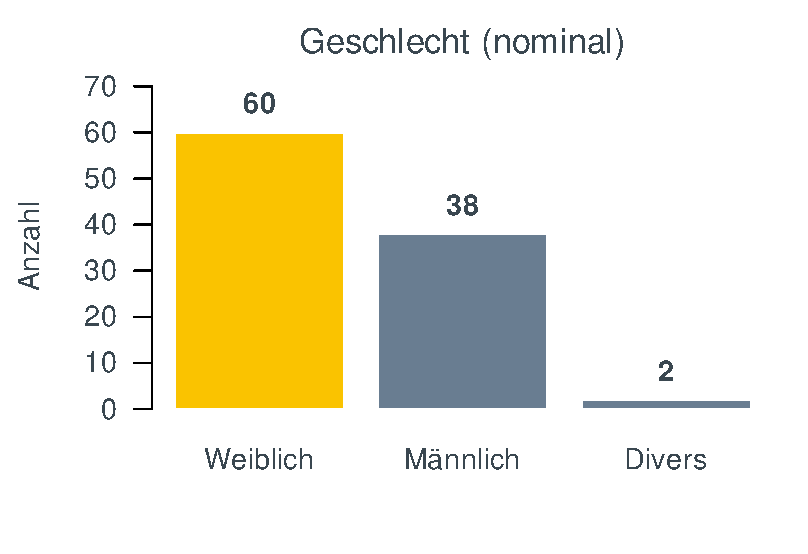
\includegraphics[width=\linewidth]{figures/ex16_geschlecht.pdf}
\end{column}
\end{columns}
\end{frame}

\begin{frame}[fragile]{\texttt{Bildung}: ordinal $\rightarrow$ Median}
\begin{columns}[T]
\begin{column}{0.5\textwidth}
\texttt{Gymnasium} $<$ \texttt{Bachelor} $<$ \texttt{Master} $<$
\texttt{Doktorat}: es gibt eine \textbf{klare Ordnung}, aber die
„Abstände`` sind nicht gleich.

\vspace{0.2cm}
$\Rightarrow$ \alert{Skalenniveau: ordinal}\\
$\Rightarrow$ Lagemass: \alert{Median} (mittlere Kategorie)

\vspace{0.2cm}
\small Mittelwert wäre \textbf{unsinnig} (was ist der Durchschnitt aus
Gymnasium und Master?).
\end{column}
\begin{column}{0.48\textwidth}
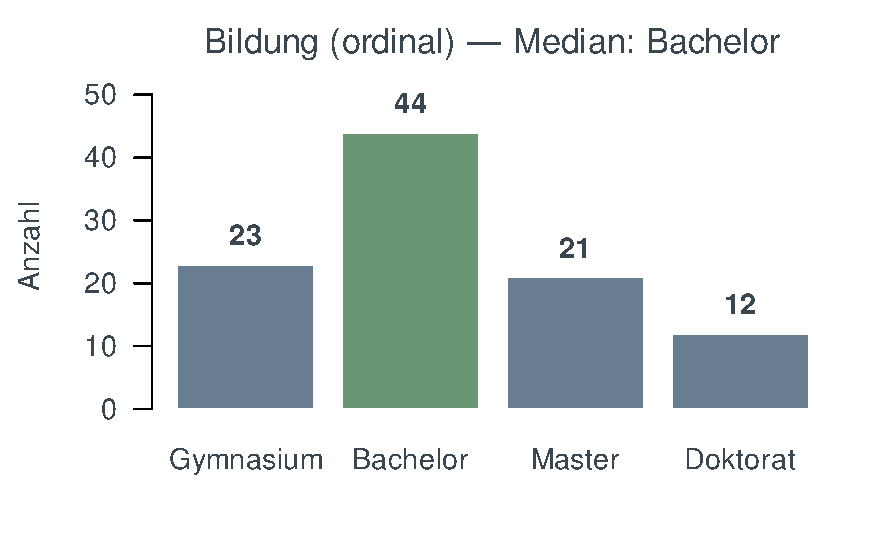
\includegraphics[width=\linewidth]{figures/ex16_bildung.pdf}
\end{column}
\end{columns}
\end{frame}

\begin{frame}[fragile]{\texttt{Bildung}: den ordinalen Median finden}
Der Median ist der Wert an Position $50{,}5$ (Mittel aus 50.\ und 51.\ Wert)
in der \textbf{geordneten} Reihe. Wir kumulieren die Häufigkeiten:

\vspace{0.2cm}
\centering
\renewcommand{\arraystretch}{1.25}
\begin{tabular}{lcccc}
\toprule
 & Gymnasium & \textbf{Bachelor} & Master & Doktorat \\
\midrule
Anzahl     & 23 & 44 & 21 & 12 \\
kumuliert  & 23 & \alert{67} & 88 & 100 \\
Positionen & 1--23 & \alert{24--67} & 68--88 & 89--100 \\
\bottomrule
\end{tabular}

\vspace{0.3cm}
Die Positionen 50 \emph{und} 51 fallen beide in \textbf{Bachelor}
(Bereich 24--67).

\vspace{0.2cm}
\centering $\Rightarrow$ Median $=$ \alert{Bachelor}
\end{frame}

\begin{frame}[fragile]{\texttt{Einkommen}: verhältnisskaliert $\rightarrow$ Mittelwert}
\begin{columns}[T]
\begin{column}{0.5\textwidth}
Einkommen in CHF: \textbf{gleiche Abstände} (1000 CHF sind überall 1000
CHF) und ein \textbf{echter Nullpunkt} (0 $=$ kein Einkommen).

\vspace{0.2cm}
$\Rightarrow$ \alert{Skalenniveau: verhältnis}\\
$\Rightarrow$ Lagemass: \alert{Mittelwert}

\begin{rcode}
round(mean(umfrage$Einkommen))
#>  83099
\end{rcode}
\centering Mittelwert $=$ \textbf{83\,099 CHF}
\end{column}
\begin{column}{0.48\textwidth}
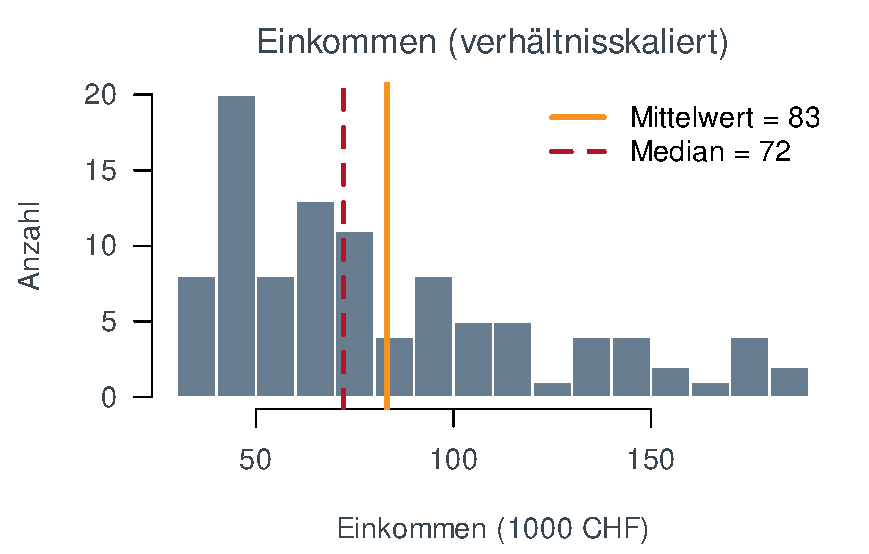
\includegraphics[width=\linewidth]{figures/ex16_einkommen.pdf}
\end{column}
\end{columns}
\vspace{0.1cm}
\small Hinweis: Die Verteilung ist rechtsschief, daher liegt der Mittelwert
(83) über dem Median (72). Gefragt ist hier der \textbf{Mittelwert}.
\end{frame}

\begin{frame}{\texttt{Bewertung}: der Sonderfall}
\texttt{Bewertung} ist eine Skala von 1 bis 10 --- eine
\textbf{Rangbewertung}.

\vspace{0.3cm}
\begin{columns}[T]
\begin{column}{0.5\textwidth}
\begin{itemize}
  \item Es gibt eine klare \textbf{Ordnung} (10 besser als 1)
  \item Aber: Ist der Abstand 1$\to$2 gleich gross wie 9$\to$10?
        Subjektiv \textbf{nicht garantiert}
\end{itemize}
\end{column}
\begin{column}{0.5\textwidth}
\begin{itemize}
  \item Höchstes \emph{gesichertes} Niveau: \alert{ordinal}
  \item Passendes Lagemass wäre der \textbf{Median} ($=6$)
\end{itemize}
\end{column}
\end{columns}

\vspace{0.3cm}
\begin{warnung}
Subjektive Ratings werden in der Praxis oft als metrisch \emph{behandelt} ---
streng genommen sind sie \textbf{ordinal}. Im Zweifel das niedrigere,
sichere Niveau angeben.
\end{warnung}
\end{frame}

\begin{frame}{Frage 16 --- Lösung auf einen Blick}
\centering
\renewcommand{\arraystretch}{1.35}
\begin{tabular}{lll}
\toprule
Variable & Höchstes Skalenniveau & Angemessenes Lagemass \\
\midrule
\texttt{Geschlecht} & nominal & Modus $=$ \textbf{Weiblich} \\
\texttt{Bildung}    & ordinal & Median $=$ \textbf{Bachelor} \\
\texttt{Einkommen}  & verhältnis (metrisch) & Mittelwert $=$ \textbf{83\,099 CHF} \\
\texttt{Bewertung}  & ordinal & (Median $=6$) \\
\bottomrule
\end{tabular}

\vspace{0.5cm}
\begin{merke}
Immer zuerst das \textbf{Skalenniveau} klären --- es entscheidet, welche
Kennzahl erlaubt ist.
\end{merke}
\end{frame}

% ============================================================
\section{Frage 17 --- Streuung, Form \& Ausreisser}
% ============================================================

\begin{frame}{Die Aufgabe}
\textbf{Datensatz \texttt{Studentenleben.xlsx}} --- 80 Studierende und ihre
Lebensstil-Daten.

\vspace{0.3cm}
Für die Variable \texttt{Lernstunden} (wöchentlich):
\begin{itemize}
  \item \alert{Lage}: Mittelwert, Median
  \item \alert{Streuung}: Standardabweichung, Interquartilsabstand (IQR)
  \item \alert{Form}: Schiefe, Verteilungsform
  \item \alert{Ausreisser}: Anzahl gemäss Tukey-Regel ($1{,}5\times$ IQR)
\end{itemize}
Für die Variable \texttt{Verkehrsmittel}: der \alert{Modus}.
\end{frame}

\begin{frame}[fragile]{Schritt 1: Daten einlesen \& Überblick}
\begin{rcode}
library(readxl)
leben <- read_excel("Studentenleben.xlsx")
lern  <- leben$Lernstunden
summary(lern)
\end{rcode}
\begin{rout}
   Min. 1st Qu.  Median    Mean 3rd Qu.    Max.
   0.80    8.40   19.30   20.34   26.98   62.50
\end{rout}
\vspace{0.2cm}
\small \texttt{summary()} liefert schon Min, Quartile, Median und Mittelwert
--- ein guter erster Überblick, bevor wir die einzelnen Kennzahlen sauber
berechnen.
\end{frame}

\begin{frame}[fragile]{Schritt 2: Lage --- Mittelwert \& Median}
\begin{columns}[T]
\begin{column}{0.52\textwidth}
\begin{rcode}
mean(lern)    # 20.34
median(lern)  # 19.30
\end{rcode}
\vspace{0.2cm}
\begin{itemize}
  \item \textbf{Mittelwert} $= 20{,}3$
  \item \textbf{Median} $= 19{,}3$
  \item Mittelwert $>$ Median --- ein erster \alert{Hinweis auf
        Rechtsschiefe}
\end{itemize}
\end{column}
\begin{column}{0.46\textwidth}
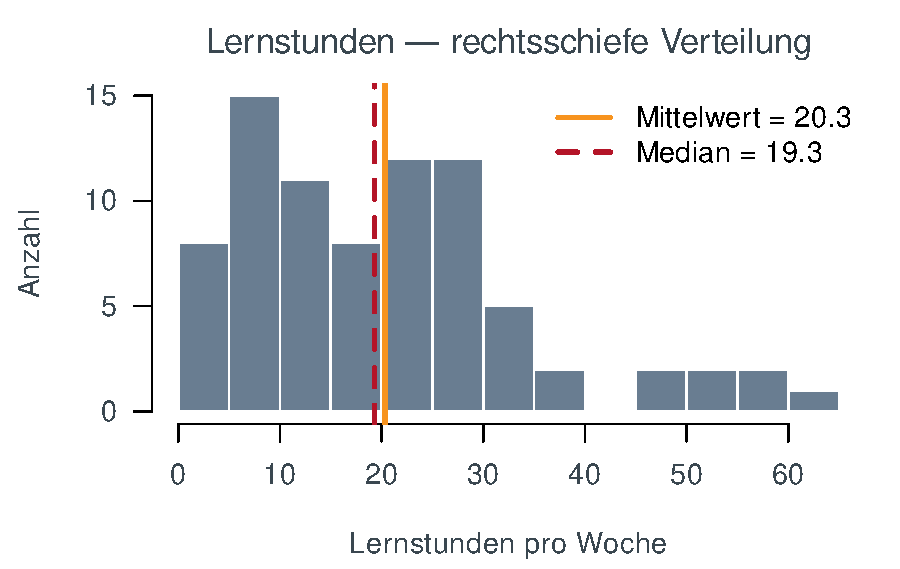
\includegraphics[width=\linewidth]{figures/ex17_hist.pdf}
\end{column}
\end{columns}
\end{frame}

\begin{frame}[fragile]{Kernkonzept: Zwei Streuungsmasse}
\begin{columns}[T]
\begin{column}{0.5\textwidth}
\textbf{Standardabweichung (SD)}
\[ s = \sqrt{\tfrac{1}{n-1}\textstyle\sum (x_i-\bar x)^2} \]
\begin{itemize}
  \item mittlere Abweichung vom \emph{Mittelwert}
  \item reagiert \alert{empfindlich} auf Ausreisser
\end{itemize}
\end{column}
\begin{column}{0.5\textwidth}
\textbf{Interquartilsabstand (IQR)}
\[ \text{IQR} = Q_3 - Q_1 \]
\begin{itemize}
  \item Breite der \emph{mittleren 50\,\%}
  \item \alert{robust} gegen Ausreisser
\end{itemize}
\end{column}
\end{columns}
\vspace{0.3cm}
\begin{rcode}
sd(lern)   # 14.0
IQR(lern)  # 18.6   (= 26.975 - 8.4)
\end{rcode}
\centering SD $= \mathbf{14{,}0}$ \qquad IQR $= \mathbf{18{,}6}$
\end{frame}

\begin{frame}{Kernkonzept: Schiefe (Skewness)}
Die \alert{Schiefe} misst die \textbf{Asymmetrie} einer Verteilung:

\vspace{0.1cm}
\begin{center}
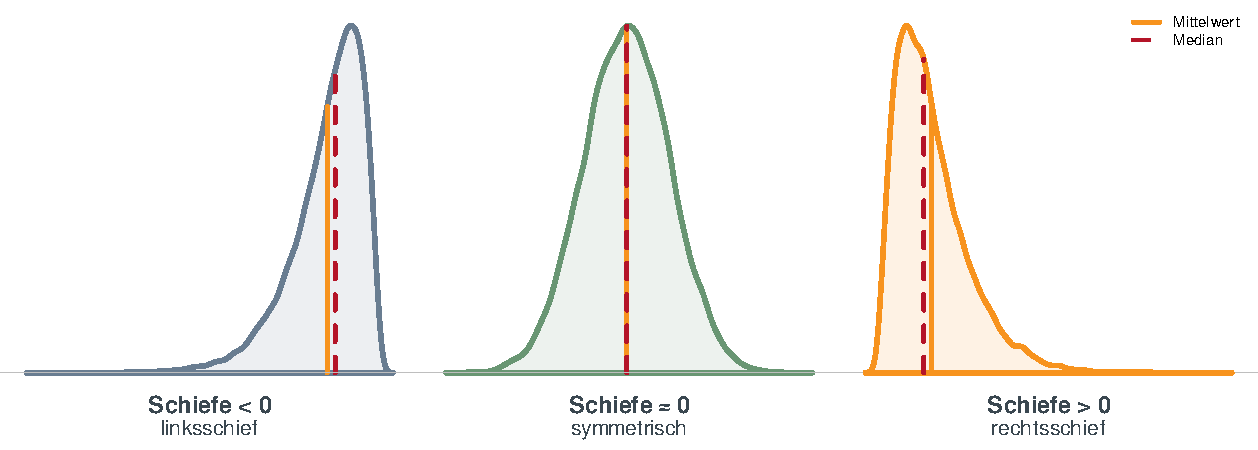
\includegraphics[width=0.96\linewidth]{figures/ex17_schiefe.pdf}
\end{center}
\vspace{0.1cm}
\begin{itemize}
  \item \textbf{rechtsschief} ($>0$): langer Schwanz nach \emph{rechts},
        Mittelwert $>$ Median
  \item \textbf{linksschief} ($<0$): langer Schwanz nach \emph{links},
        Mittelwert $<$ Median
\end{itemize}
\end{frame}

\begin{frame}[fragile]{Schritt 3: Schiefe \& Verteilungsform}
\begin{columns}[T]
\begin{column}{0.5\textwidth}
\begin{rcode}
library(e1071)
skewness(lern)
#>  1.05
\end{rcode}
\vspace{0.2cm}
\begin{itemize}
  \item Schiefe $\approx \mathbf{1{,}05} > 0$
  \item langer Schwanz nach rechts (wenige Viel-Lerner)
  \item Mittelwert (20{,}3) $>$ Median (19{,}3) bestätigt das
\end{itemize}
\centering $\Rightarrow$ \alert{rechtsschiefe Verteilung}
\end{column}
\begin{column}{0.46\textwidth}
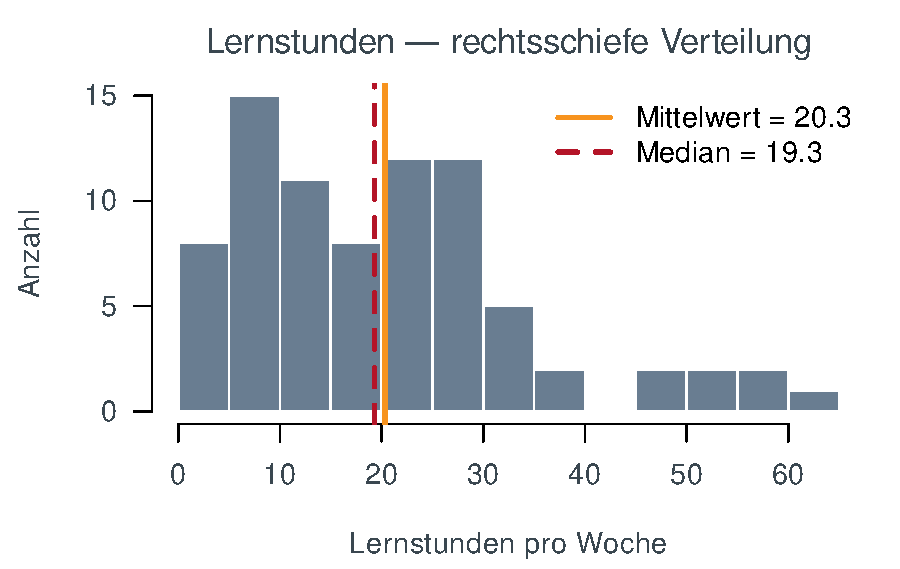
\includegraphics[width=\linewidth]{figures/ex17_hist.pdf}
\end{column}
\end{columns}
\vspace{0.1cm}
\small\textit{Wichtig ist nicht die exakte Zahl, sondern das
\textbf{Vorzeichen}:} positiv $\Rightarrow$ rechtsschief.
\end{frame}

\begin{frame}{Kernkonzept: Die Tukey-Ausreisserregel}
Ein Wert gilt als \alert{Ausreisser}, wenn er ausserhalb der „Zäune``
liegt, die $1{,}5\times$ IQR über $Q_3$ bzw.\ unter $Q_1$ gesetzt werden:

\vspace{0.2cm}
\[
  \text{unterer Zaun} = Q_1 - 1{,}5\cdot\text{IQR}
  \qquad
  \text{oberer Zaun} = Q_3 + 1{,}5\cdot\text{IQR}
\]

\vspace{0.2cm}
\begin{center}
\begin{tikzpicture}[font=\scriptsize, scale=1]
  \draw[thick] (1,0) -- (9,0);
  \filldraw[LitmusPrimary!30, draw=LitmusPrimary, thick] (3,-0.35) rectangle (6,0.35);
  \draw[thick] (4.5,-0.35) -- (4.5,0.35);                    % Median
  \draw[thick] (3,0) -- (1.8,0); \draw[thick] (6,0) -- (8,0); % Whisker
  \draw[thick] (1.8,-0.2) -- (1.8,0.2); \draw[thick] (8,-0.2) -- (8,0.2);
  \node at (3,0.65) {$Q_1$}; \node at (6,0.65) {$Q_3$};
  \node[LitmusAlert] at (8,-0.6) {oberer Zaun};
  \filldraw[LitmusIncorrect] (8.7,0) circle (2pt);
  \node[LitmusIncorrect] at (8.7,0.5) {Ausreisser};
\end{tikzpicture}
\end{center}
\vspace{0.1cm}
\centering\small Genau diese Regel zeichnet R automatisch im
\textbf{Boxplot}.
\end{frame}

\begin{frame}[fragile]{Schritt 4: Ausreisser zählen}
\begin{columns}[T]
\begin{column}{0.5\textwidth}
\begin{rcode}
Q <- quantile(lern, c(.25,.75))
iqr <- Q[2] - Q[1]          # 18.6
zaun_oben <- Q[2] + 1.5*iqr # 54.8
zaun_unten<- Q[1] - 1.5*iqr # -19.5
sum(lern > zaun_oben |
    lern < zaun_unten)
#>  3
\end{rcode}
\vspace{0.1cm}
\begin{itemize}
  \item oberer Zaun $= 54{,}8$, unterer $= -19{,}5$
  \item 3 Werte darüber: \textbf{57, 57, 62{,}5}
\end{itemize}
\centering $\Rightarrow$ \alert{3 Ausreisser}
\end{column}
\begin{column}{0.48\textwidth}
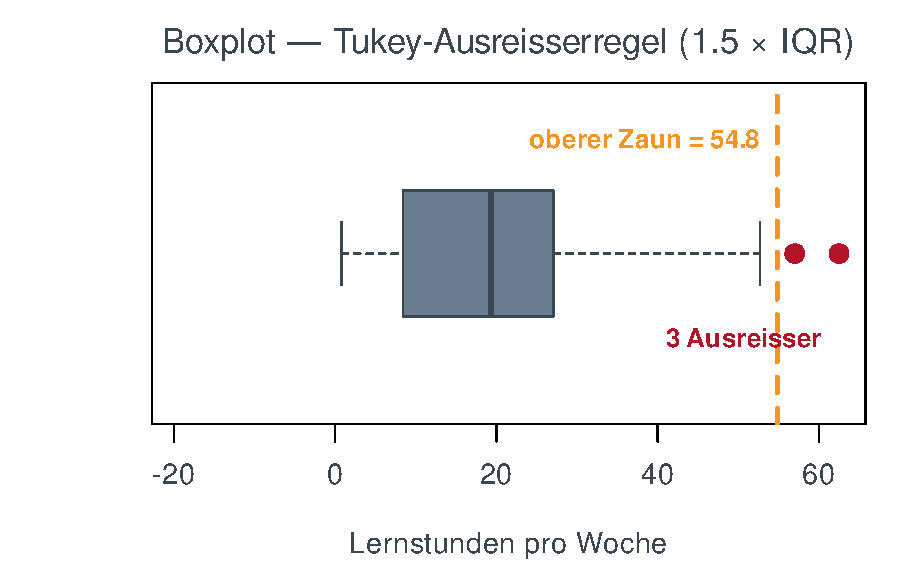
\includegraphics[width=\linewidth]{figures/ex17_box.pdf}
\end{column}
\end{columns}
\end{frame}

\begin{frame}[fragile]{\texttt{Verkehrsmittel}: nominal $\rightarrow$ Modus}
\begin{columns}[T]
\begin{column}{0.5\textwidth}
\texttt{Verkehrsmittel} ist \textbf{nominal} --- also ist der
\alert{Modus} (häufigste Kategorie) das einzig sinnvolle Lagemass.

\begin{rcode}
table(leben$Verkehrsmittel)
#> Auto Fahrrad   ÖV Zu Fuss
#>   25      11   36       8
\end{rcode}
\centering Modus $=$ \textbf{ÖV} (36 von 80)
\end{column}
\begin{column}{0.48\textwidth}
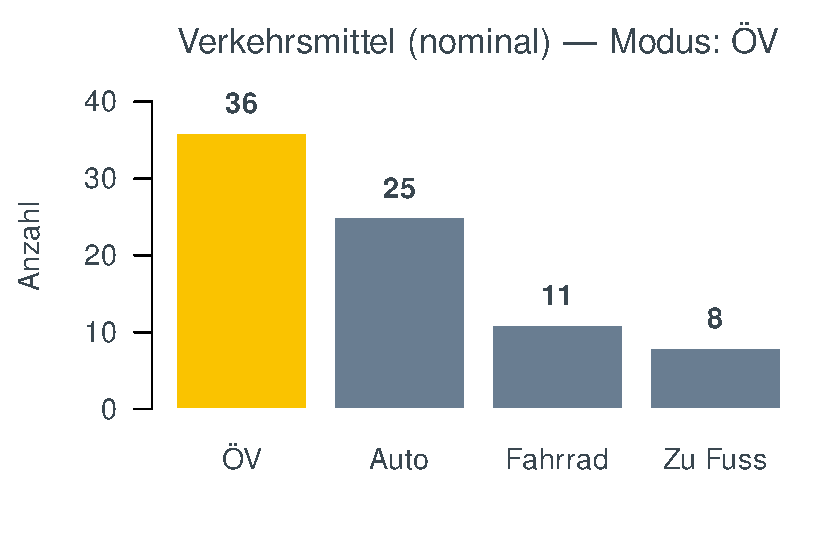
\includegraphics[width=\linewidth]{figures/ex17_verkehr.pdf}
\end{column}
\end{columns}
\end{frame}

\begin{frame}{Frage 17 --- Lösung auf einen Blick}
\centering
\renewcommand{\arraystretch}{1.3}
\begin{tabular}{ll}
\toprule
Kennzahl (\texttt{Lernstunden}) & Wert \\
\midrule
Mittelwert            & \textbf{20{,}3} \\
Median                & \textbf{19{,}3} \\
Standardabweichung    & \textbf{14{,}0} \\
Interquartilsabstand (IQR) & \textbf{18{,}6} \\
Schiefe               & \textbf{1{,}05} \\
Verteilungsform       & \textbf{rechtsschief} \\
Ausreisser (Tukey $1{,}5\times$IQR) & \textbf{3} \\
\midrule
Modus \texttt{Verkehrsmittel} & \textbf{ÖV} \\
\bottomrule
\end{tabular}
\end{frame}

% ============================================================
\section{Frage 18 --- Bootstrap-CI für eine Anteilsdifferenz}
% ============================================================

\begin{frame}{Die Aufgabe}
\textbf{Datensatz \texttt{ImpfabsichtUmfrage.xlsx}} --- 250 Personen, zufällig
auf zwei Gruppen verteilt:
\begin{itemize}
  \item \texttt{Behandlung}: sah ein informatives Aufklärungsvideo
  \item \texttt{Kontrolle}: sah ein neutrales Kontrollvideo
\end{itemize}
\texttt{Impfabsicht} ist binär kodiert ($1 =$ ja, $0 =$ nein).

\vspace{0.3cm}
Gesucht ist die Differenz
$\hat p_{\text{diff}} = \hat p_{\text{Behandlung}} - \hat p_{\text{Kontrolle}}$
und ein \alert{95\%-Bootstrap-Konfidenzintervall} (5000 Stichproben).
Ist der Unterschied \alert{signifikant}?
\end{frame}

\begin{frame}{Kernkonzept: Warum Bootstrap für eine Differenz?}
Wir haben \emph{eine} Stichprobe und schätzen daraus \emph{einen} Wert
$\hat p_{\text{diff}}$. Aber wie sicher ist dieser?

\vspace{0.2cm}
\begin{center}
\begin{tikzpicture}[>=Stealth, font=\small,
   box/.style={draw, rounded corners, minimum width=2.7cm, minimum height=1.1cm,
               text width=2.5cm, align=center}]
  \node[box, fill=LitmusPrimary!10]   (d) at (0,0)   {Daten\\($n=250$)};
  \node[box, fill=LitmusSecondary!25] (s) at (4.4,0) {Stichprobe\\\emph{mit Zurücklegen}};
  \node[box, fill=LitmusAccent!12]    (m) at (8.8,0) {$\hat p_{\text{diff}}$ berechnen};
  \draw[->,thick] (d)--(s) node[midway,above,font=\scriptsize]{ziehen};
  \draw[->,thick] (s)--(m) node[midway,above,font=\scriptsize]{Differenz};
  \draw[->,thick,LitmusIncorrect] (m.south) -- ++(0,-0.7) -| (d.south)
    node[midway,below=2pt,font=\scriptsize,LitmusIncorrect]{5000$\times$ wiederholen};
\end{tikzpicture}
\end{center}
\vspace{0.2cm}
Die \alert{mittleren 95\,\%} der 5000 simulierten Differenzen bilden das
Konfidenzintervall. \textbf{Enthält es die 0 nicht}, ist der Unterschied
signifikant.
\end{frame}

\begin{frame}[fragile]{Schritt 1: Anteile je Gruppe}
\begin{columns}[T]
\begin{column}{0.5\textwidth}
\begin{rcode}
library(readxl)
imp <- read_excel(
  "ImpfabsichtUmfrage.xlsx")
# Anteile je Gruppe
tapply(imp$Impfabsicht,
       imp$Gruppe, mean)
#> Behandlung  Kontrolle
#>     0.692      0.431
\end{rcode}
\centering
$\hat p_{\text{diff}} = 0{,}692 - 0{,}431 = \mathbf{0{,}26}$
\end{column}
\begin{column}{0.48\textwidth}
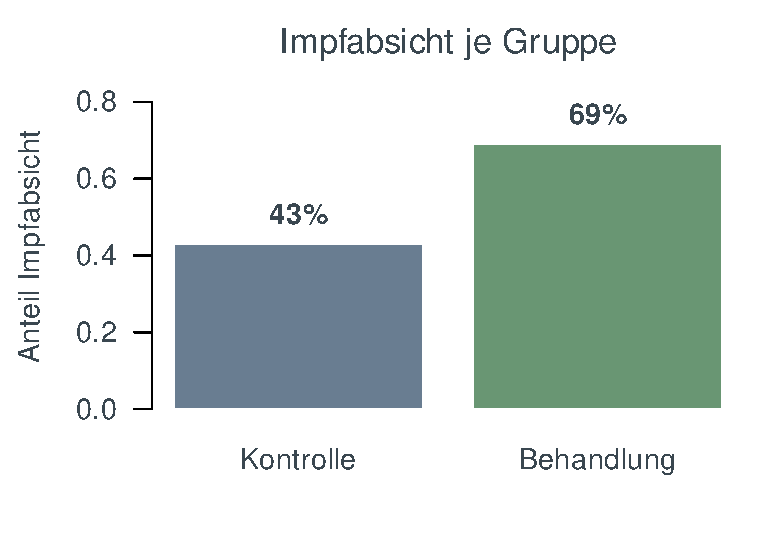
\includegraphics[width=\linewidth]{figures/ex18_anteile.pdf}
\end{column}
\end{columns}
\end{frame}

\begin{frame}[fragile]{Schritt 2: Bootstrap mit \texttt{mosaic::do()}}
\begin{columns}[T]
\begin{column}{0.5\textwidth}
\begin{rcode}
library(mosaic)
set.seed(2024)
pdiff <- function(d)
  mean(d$Impfabsicht[
        d$Gruppe=="Behandlung"]) -
  mean(d$Impfabsicht[
        d$Gruppe=="Kontrolle"])
boot <- do(5000) *
        pdiff(resample(imp))
quantile(boot$pdiff,
         c(.025, .975))
#>   0.14    0.38
\end{rcode}
\end{column}
\begin{column}{0.48\textwidth}
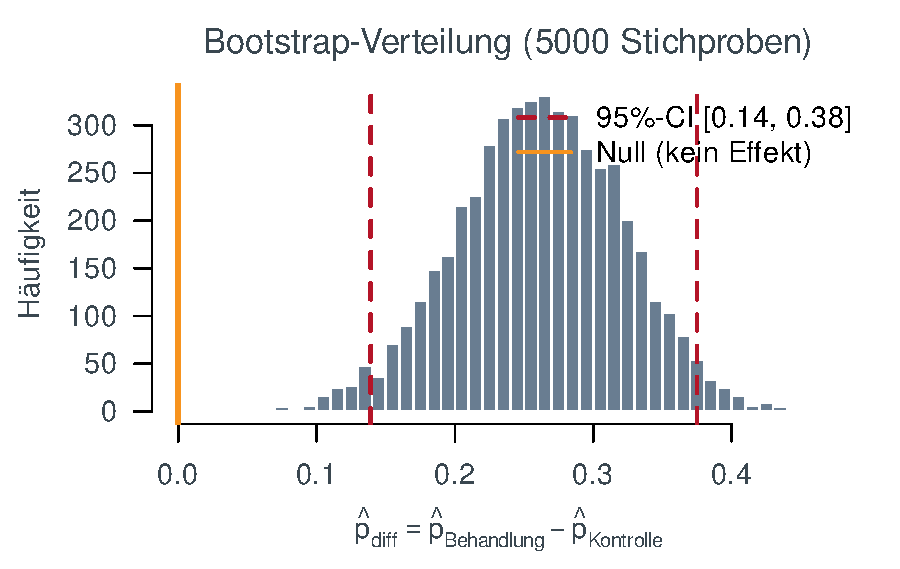
\includegraphics[width=\linewidth]{figures/ex18_boot.pdf}
\end{column}
\end{columns}
\end{frame}

\begin{frame}{Frage 18 --- Lösung \& Interpretation}
\centering
\renewcommand{\arraystretch}{1.3}
\begin{tabular}{ll}
\toprule
Untere Grenze des 95\%-CI & \textbf{0{,}14} \\
Obere Grenze des 95\%-CI  & \textbf{0{,}38} \\
Signifikant? & \textbf{Ja} \\
\bottomrule
\end{tabular}

\vspace{0.4cm}
\begin{merke}
Das Intervall $[0{,}14;\ 0{,}38]$ enthält die \textbf{0 nicht} und liegt
ganz im Positiven. Das Aufklärungsvideo erhöht die Impfbereitschaft also
\alert{statistisch signifikant} --- um geschätzte 14 bis 38 Prozentpunkte.
\end{merke}
\end{frame}

% ============================================================
\section{Frage 19 --- Ein Streudiagramm lesen}
% ============================================================

\begin{frame}{Die Aufgabe}
\begin{columns}[T]
\begin{column}{0.52\textwidth}
Ein Streudiagramm ist gegeben. Welche Aussagen sind richtig?
\textbf{Ohne Rechnen} --- nur fundiert \emph{abschätzen}:

\vspace{0.2cm}
\small
\begin{itemize}
  \item[a.] $|r| \ge 0{,}8$
  \item[b.] Für $X=-0{,}8$ erwartet man $Y \approx 1{,}9$
  \item[c.] Das Streudiagramm ist standardisiert
  \item[d.] Mittelwert von $X$ ist ungefähr $0$
  \item[e.] Standardabweichung von $X$ ist mindestens $5$
\end{itemize}
\end{column}
\begin{column}{0.46\textwidth}
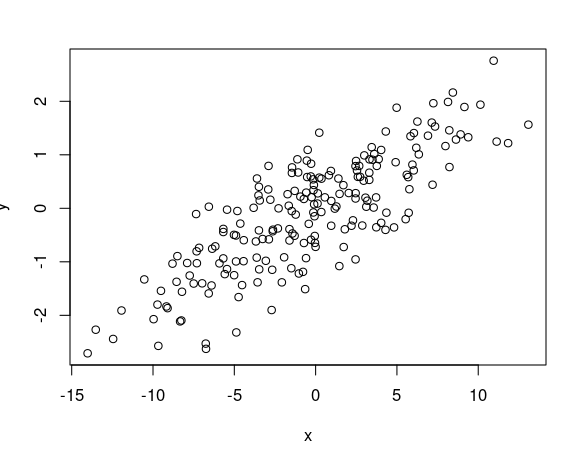
\includegraphics[width=\linewidth]{figures/ex19_scatter.png}
\end{column}
\end{columns}
\end{frame}

\begin{frame}{Kernkonzept: Was man aus den Achsen abliest}
\begin{columns}[T]
\begin{column}{0.46\textwidth}
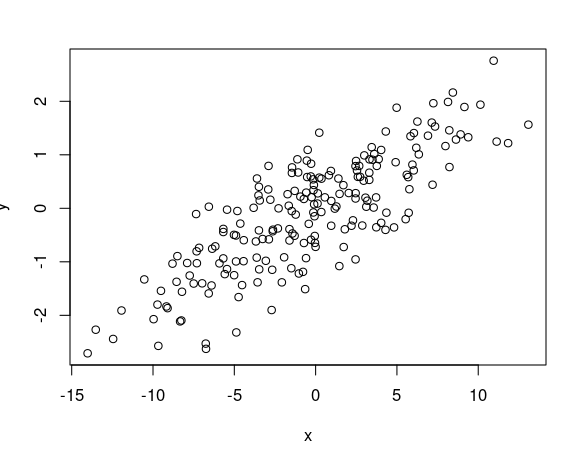
\includegraphics[width=\linewidth]{figures/ex19_scatter.png}
\end{column}
\begin{column}{0.5\textwidth}
\textbf{Achsenbereiche verraten Lage \& Streuung:}
\begin{itemize}
  \item $X$ läuft von $\approx -15$ bis $+12$, Wolke um $0$ zentriert
        $\Rightarrow$ Mittelwert $\approx 0$
  \item Spannweite $\approx 27$; Faustregel SD $\approx$ Spannweite$/4$
        $\Rightarrow$ SD$_X \approx 5$--$6$
  \item $Y$ läuft nur von $-2{,}5$ bis $+2{,}5$ $\Rightarrow$ sieht
        standardisiert aus ($\bar y \approx 0$, $s_y \approx 1$)
  \item $X$ ist \alert{nicht} standardisiert (SD $\gg 1$)
\end{itemize}
\end{column}
\end{columns}
\end{frame}

\begin{frame}{Frage 19 --- die Aussagen einzeln prüfen}
\renewcommand{\arraystretch}{1.3}
\centering
\begin{tabular}{clp{6.4cm}}
\toprule
 & Aussage & Beurteilung \\
\midrule
a. & $|r|\ge 0{,}8$ & \textcolor{LitmusAccent}{\textbf{richtig}}: enge, klar steigende Wolke \\
b. & $X=-0{,}8 \Rightarrow Y\approx 1{,}9$ & \textcolor{LitmusIncorrect}{\textbf{falsch}}: bei $X\approx 0$ ist $Y\approx 0$, nicht $1{,}9$ \\
c. & standardisiert & \textcolor{LitmusIncorrect}{\textbf{falsch}}: nur $Y$, $X$ hat SD $\approx 5$ \\
d. & $\bar X \approx 0$ & \textcolor{LitmusAccent}{\textbf{richtig}}: Wolke um $0$ zentriert \\
e. & SD$_X \ge 5$ & \textcolor{LitmusAccent}{\textbf{richtig}}: Spannweite $\approx 27$ \\
\bottomrule
\end{tabular}

\vspace{0.3cm}
\begin{merke}
Richtige Antworten: \alert{a, d, e}. Schlüssel: Achsenbereiche zeigen Lage
und Streuung, der Punkt $(0,0)$ die Regressionsmitte.
\end{merke}
\end{frame}

% ============================================================
\section{Frage 20 --- Einfache lineare Regression}
% ============================================================

\begin{frame}{Die Aufgabe}
\textbf{Datensatz \texttt{Immobilienpreise.xlsx}} --- 120 verkaufte
Einfamilienhäuser.
\begin{itemize}
  \item \texttt{Quadratmeter}: Wohnfläche in m$^2$
  \item \texttt{Preis\_kCHF}: Verkaufspreis in 1000 CHF
\end{itemize}

\vspace{0.2cm}
Einfache lineare Regression \texttt{Preis\_kCHF $\sim$ Quadratmeter}.
Gesucht:
\begin{itemize}
  \item \alert{Steigung} (2 Dezimalstellen) und \alert{$R^2$} (3 Dezimalstellen)
  \item \alert{95\%-Konfidenzintervall} für die Steigung
  \item Ist die Steigung \alert{signifikant} von Null verschieden
        ($\alpha = 0{,}05$)?
\end{itemize}
\end{frame}

\begin{frame}[fragile]{Schritt 1: Modell schätzen}
\begin{columns}[T]
\begin{column}{0.5\textwidth}
\begin{rcode}
imm <- read_excel(
  "Immobilienpreise.xlsx")
mod <- lm(Preis_kCHF ~
          Quadratmeter, data = imm)
summary(mod)
\end{rcode}
\begin{rout}
            Estimate Std.Err t value
(Intercept) -12.7338  19.20   -0.66
Quadratmeter  4.1807   0.102   40.8
Multiple R-squared:  0.9339
\end{rout}
\end{column}
\begin{column}{0.48\textwidth}
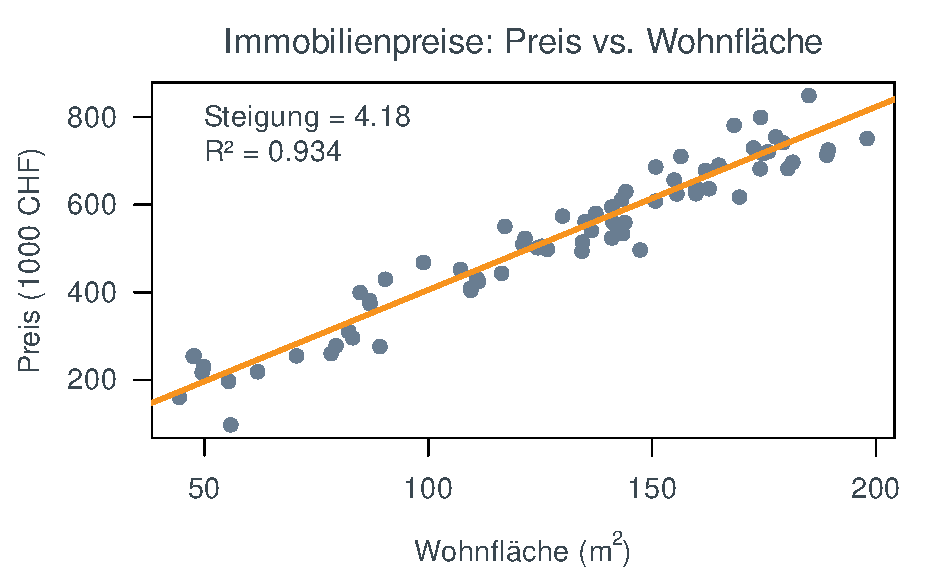
\includegraphics[width=\linewidth]{figures/ex20_scatter.pdf}
\end{column}
\end{columns}
\vspace{0.1cm}
\centering\small
Steigung $= \mathbf{4{,}18}$ \quad $R^2 = \mathbf{0{,}934}$ \quad
(pro m$^2$ rund 4180 CHF mehr)
\end{frame}

\begin{frame}[fragile]{Schritt 2: Konfidenzintervall \& Signifikanz}
\begin{rcode}
confint(mod, "Quadratmeter")          # 95%-CI der Steigung
#>               2.5 %   97.5 %
#> Quadratmeter  3.978    4.384
\end{rcode}
\vspace{0.2cm}
\begin{columns}[T]
\begin{column}{0.5\textwidth}
\begin{itemize}
  \item 95\%-CI der Steigung: \alert{$[3{,}98;\ 4{,}38]$}
  \item das Intervall liegt klar \textbf{über 0}
  \item $t = 40{,}8$, $p < 0{,}001$
\end{itemize}
\end{column}
\begin{column}{0.5\textwidth}
\begin{merke}
Da das CI die 0 nicht enthält (und $p < 0{,}05$), ist die Steigung
\alert{signifikant} --- Wohnfläche erklärt den Preis sehr deutlich.
\end{merke}
\end{column}
\end{columns}
\end{frame}

\begin{frame}{Frage 20 --- Lösung auf einen Blick}
\centering
\renewcommand{\arraystretch}{1.3}
\begin{tabular}{ll}
\toprule
Kennzahl & Wert \\
\midrule
Steigung der Regressionsgeraden & \textbf{4{,}18} \\
Bestimmtheitsmass $R^2$         & \textbf{0{,}934} \\
95\%-CI Steigung -- untere Grenze & \textbf{3{,}98} \\
95\%-CI Steigung -- obere Grenze  & \textbf{4{,}38} \\
Signifikant von Null verschieden? & \textbf{Ja} \\
\bottomrule
\end{tabular}
\end{frame}

% ============================================================
\section{Zusammenfassung}
% ============================================================

\begin{frame}{Die grossen Ideen}
\begin{columns}[T]
\begin{column}{0.32\textwidth}
\begin{konzept}[Fragen 15--17]
\textbf{Beschreiben}\\[3pt]
Boxplots lesen; Skalenniveau $\to$ Lagemass; Lage, Streuung (SD/IQR) und
Form (Schiefe, Tukey-Ausreisser).
\end{konzept}
\end{column}
\begin{column}{0.32\textwidth}
\begin{konzept}[Frage 18]
\textbf{Schliessen}\\[3pt]
Bootstrap-CI für eine Anteilsdifferenz. Enthält das CI die 0 nicht
$\Rightarrow$ signifikant.
\end{konzept}
\end{column}
\begin{column}{0.32\textwidth}
\begin{konzept}[Fragen 19 \& 20]
\textbf{Zusammenhänge}\\[3pt]
Streudiagramm abschätzen (Korrelation, Lage, Streuung) und Regression
schätzen ($R^2$, CI der Steigung).
\end{konzept}
\end{column}
\end{columns}
\vspace{0.4cm}
\begin{merke}[Roter Faden]
Erst \textbf{beschreiben} (Skalenniveau, Lage, Streuung, Form), dann
\textbf{Unsicherheit beziffern} (Bootstrap) und \textbf{Zusammenhänge
modellieren} (Regression).
\end{merke}
\end{frame}

\begin{frame}[standout]
Fragen?
\end{frame}

\end{document}
